\documentclass[a4paper,10pt]{article}
\usepackage{ctex}
\usepackage{graphicx}
\usepackage{subfigure}
\usepackage{geometry}
\usepackage{array}
\usepackage{booktabs}

%opening
\geometry{left=2.0cm,right=2.0cm,top=2.5cm,bottom=2.5cm}
\title{网络对战国际象棋设计文档}
\author{计86\ 孔祥哲\ 2018011997}
\date{}

\begin{document}

\maketitle

\section{使用简介}
\subsection{功能}
\begin{itemize}
 \item 实现了国际象棋的基本规则(除了吃过路兵)
 \item 实现了网络联机和本地连接对战
 \item 实现了残局的保存和载入
\end{itemize}
\subsection{界面}
\begin{figure}[htbp]
 \centering
 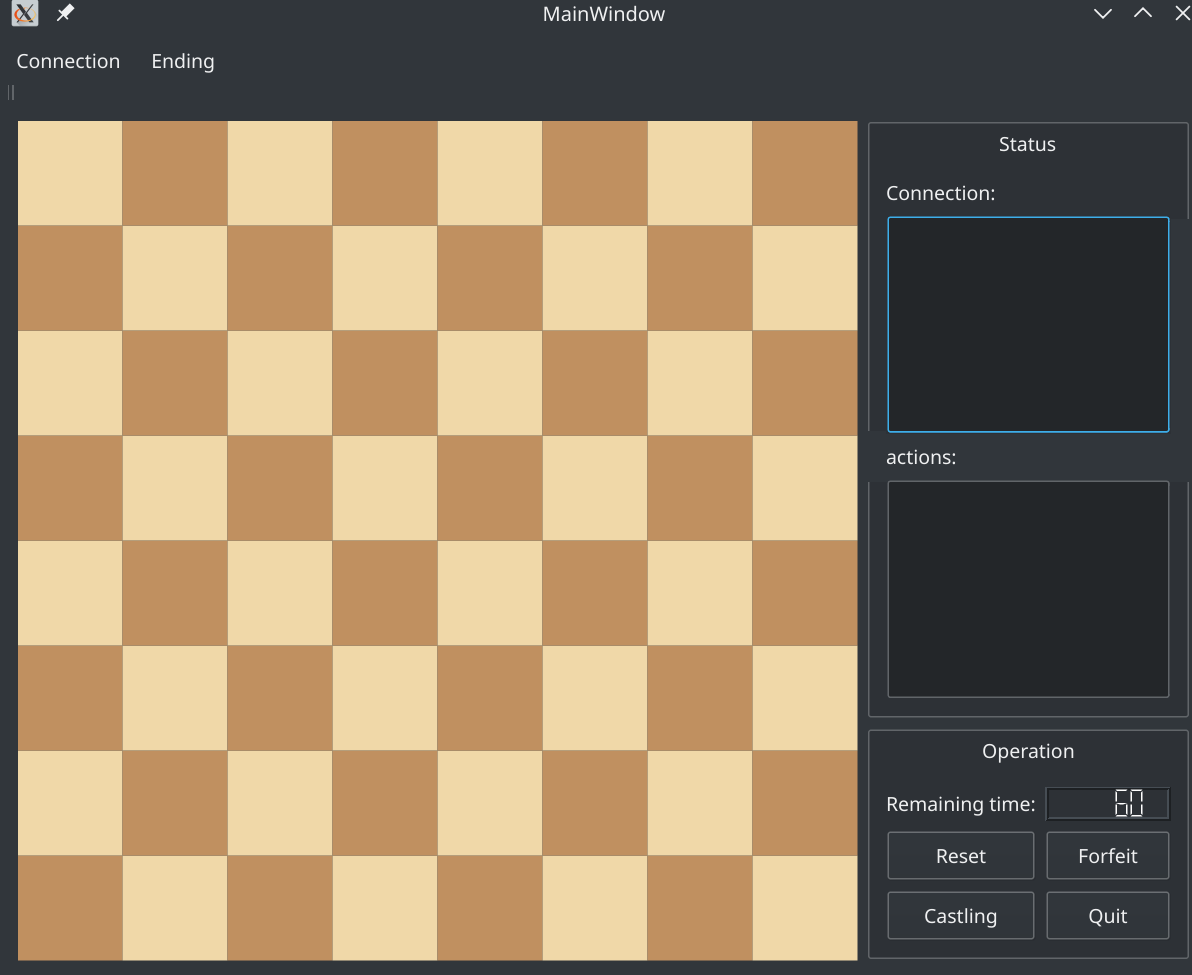
\includegraphics[width=.8\textwidth]{ui.png}
 \caption{UI界面}
 \label{fig1}
\end{figure}
左上方的connection选项中包含启动服务端(Alt+S)、客户端(Alt+W)、断开连接(无快捷键)以及退出程序(Esc)的选项,Ending菜单项中包含保存(Ctrl+S)和载入(Ctrl+L)残局的选项。\par
\begin{figure}[htbp]
 \centering
 
 %\subfigure[connection菜单]{
        \begin{minipage}[b]{.49\textwidth}
        \centering
        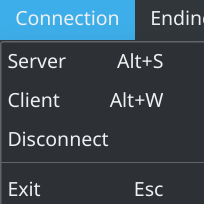
\includegraphics[width=.5\textwidth]{connection.png}
        \caption{connection菜单}
        \label{fig2}
        \end{minipage}
%}
%\subfigure[ending菜单]{
        \begin{minipage}[b]{.49\textwidth}
        \centering
        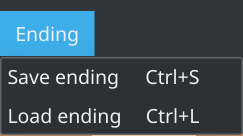
\includegraphics[width=.5\textwidth]{ending.png}
        \caption{ending菜单}
        \label{fig3}
        \end{minipage}
%}

\end{figure}

右侧状态栏中,connection标注的文本框会显示当前的连接状态,而action标注的文本框会显示该局两方的行动指令。\par
右下LCD数字显示表示该步棋手剩余决策时间。四个按钮分别对应重置棋局(只有服务端可以)、投降、王车易位、退出。\par
\begin{figure}[htbp]
 \centering
 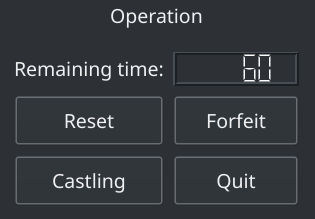
\includegraphics[width=.3\textwidth]{buttons.png}
 \caption{时间与按钮}
 \label{fig4}
\end{figure}
        \subsection{使用帮助}
                \subsubsection{服务端}
                        \begin{enumerate}
                                \item 在connection菜单中点击Server选项
                                \item 在跳出的对话框中选择默认的IP地址(如果联网会默认本机IP地址,如果没有联网会默认回送地址127.0.0.1)并确认
                                        \begin{figure}[htbp]
                                                \centering
                                                \begin{minipage}{.3\textwidth}
                                                        \centering
                                                        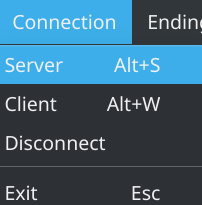
\includegraphics[width=.7\textwidth]{server.png}
                                                        \caption{Server选项}
                                                        \label{fig5}
                                                \end{minipage}
                                                \begin{minipage}{.3\textwidth}
                                                        \centering
                                                        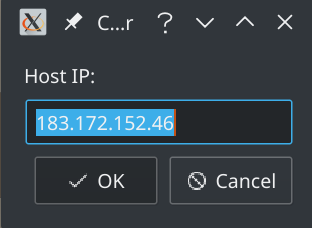
\includegraphics[width=.7\textwidth]{serverip.png}
                                                        \caption{Server IP地址}
                                                        \label{fig6}
                                                \end{minipage}
                                                \begin{minipage}{.3\textwidth}
                                                        \centering
                                                        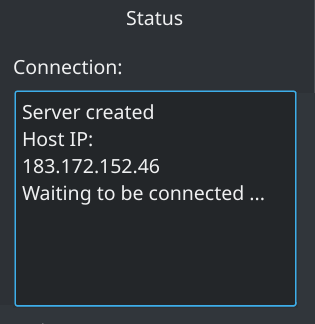
\includegraphics[width=.7\textwidth]{serverwaiting.png}
                                                        \caption{等待连接}
                                                        \label{fig7}
                                                \end{minipage}
                                        \end{figure}

                                \item connection文本框会显示服务端进入等待连接状态。此时只需等待客户端进行连接,也可以在connection菜单栏中点击disconnect取消服务器的创建
                                \item 连接成功后服务器端会跳出选择开局的对话框,先选择进行新局或者载入残局,再选择己方颜色。全部选择完成之后两方即可开始对弈
                                        \begin{figure}[htbp]
                                                \subfigure[选择开始方式]{
                                                        \begin{minipage}{.48\textwidth}
                                                                \centering
                                                                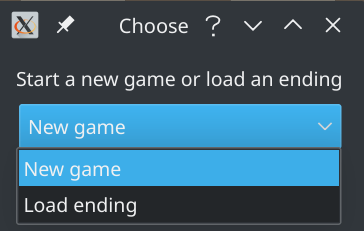
\includegraphics[width=.5\textwidth]{start.png}
                                                        \end{minipage}
                                                }
                                                \subfigure[选择颜色]{
                                                        \begin{minipage}{.48\textwidth}
                                                                \centering
                                                                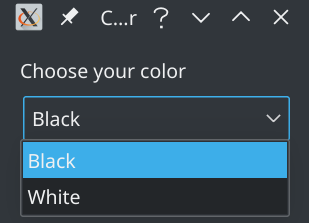
\includegraphics[width=.5\textwidth]{color.png}
                                                        \end{minipage}
                                                }
                                                \subfigure[开始对弈]{
                                                        \begin{minipage}{1\textwidth}
                                                                \centering
                                                                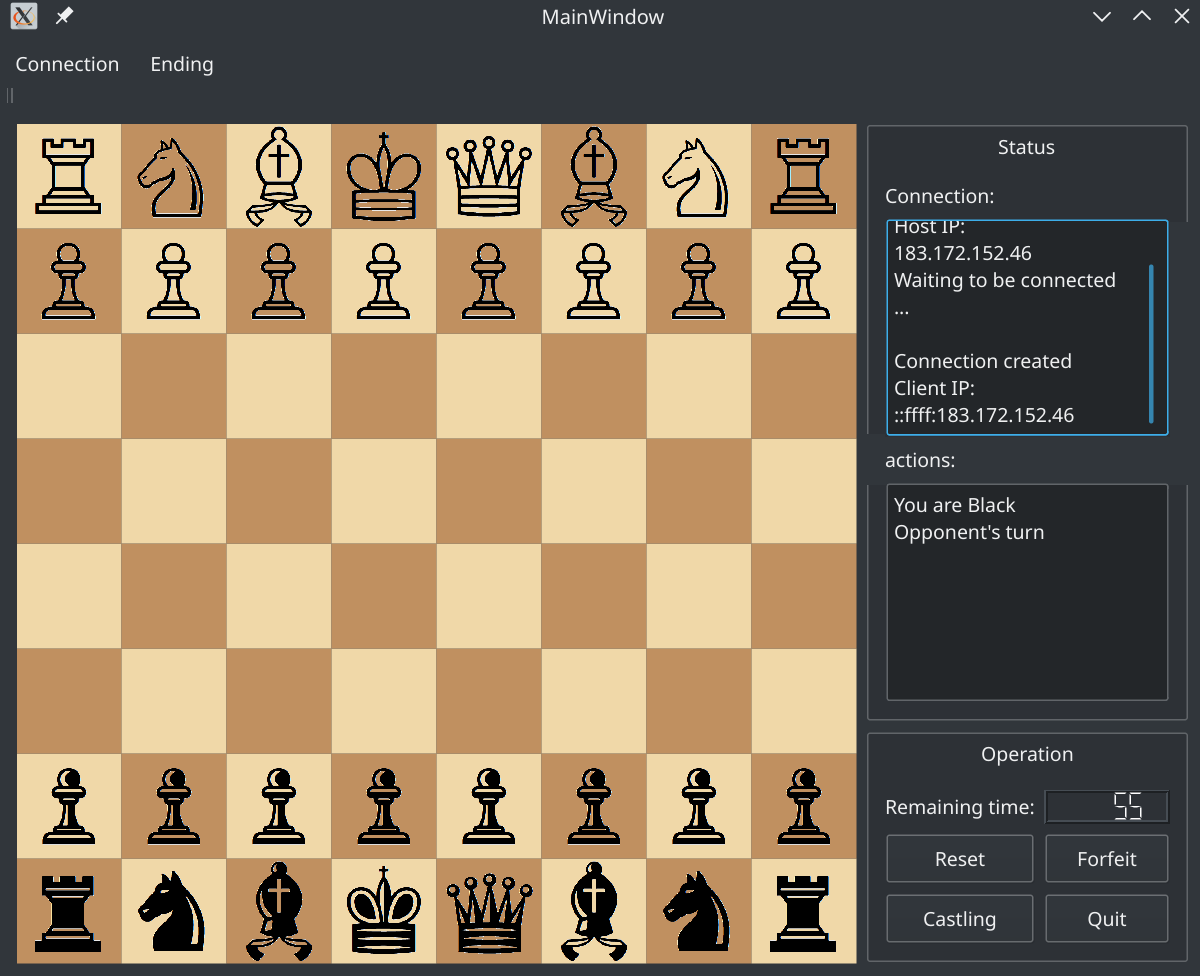
\includegraphics[width=.5\textwidth]{play.png}
                                                        \end{minipage}
                                                }
                                        \end{figure}
                        \end{enumerate}
                \subsubsection{客户端}
                        \begin{enumerate}
                         \item 在connection菜单中点击Client选项
                         \item 在跳出的对话框中输入要连接的服务端的IP地址,等待一段时间后,如果成功则会在文本框中显示信息,否则会跳出连接失败的对话框
                                \begin{figure}[htbp]
                                        \centering
                                        \subfigure[连接成功]{
                                                \begin{minipage}{.3\textwidth}
                                                        \centering
                                                        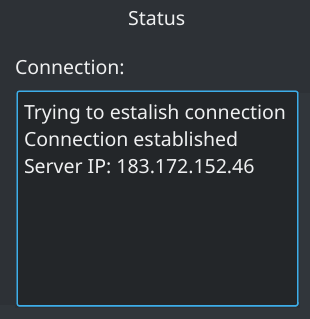
\includegraphics[width=.7\textwidth]{clientsuccess.png}
                                                \end{minipage}
                                        }
                                        \subfigure[连接失败1]{
                                                \begin{minipage}{.3\textwidth}
                                                        \centering
                                                        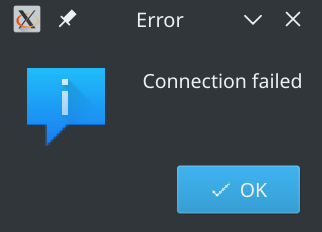
\includegraphics[width=.7\textwidth]{clientfaileddialog.png}
                                                \end{minipage}
                                        }
                                        \subfigure[连接失败2]{
                                                \begin{minipage}{.3\textwidth}
                                                        \centering
                                                        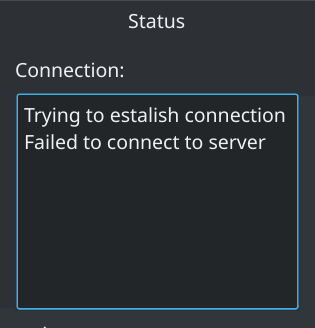
\includegraphics[width=.7\textwidth]{clientfailedtext.png}
                                                \end{minipage}
                                        }
                                \end{figure}
                         \item 连接成功后只需等待服务端选择好开局信息即可对弈
                        \end{enumerate}
                \subsubsection{保存和载入残局}
                        \begin{itemize}
                         \item 在任何时候都可通过ending菜单栏中的Save ending一项保存当前局势,也可通过Ctrl+S快捷键保存
                         \item 在连接创建完成和时服务端可选择载入残局,也可在保持连接的状态下通过服务端Reset按钮或者ending菜单栏中的Load ending(快捷键为Ctrl+L)进行残局载入
                        \end{itemize}
                \subsubsection{游戏操作}
                        \begin{itemize}
                         \item 暗黄色指代当前选中的己方棋子
                         \item 亮黄色为可以前进的位置
                         \item 红色为选中的敌方棋子或者提示可以吃
                         \item 王车易位使用专用的按钮
                        \end{itemize}
                        \begin{figure}[htbp]
                                \centering
                                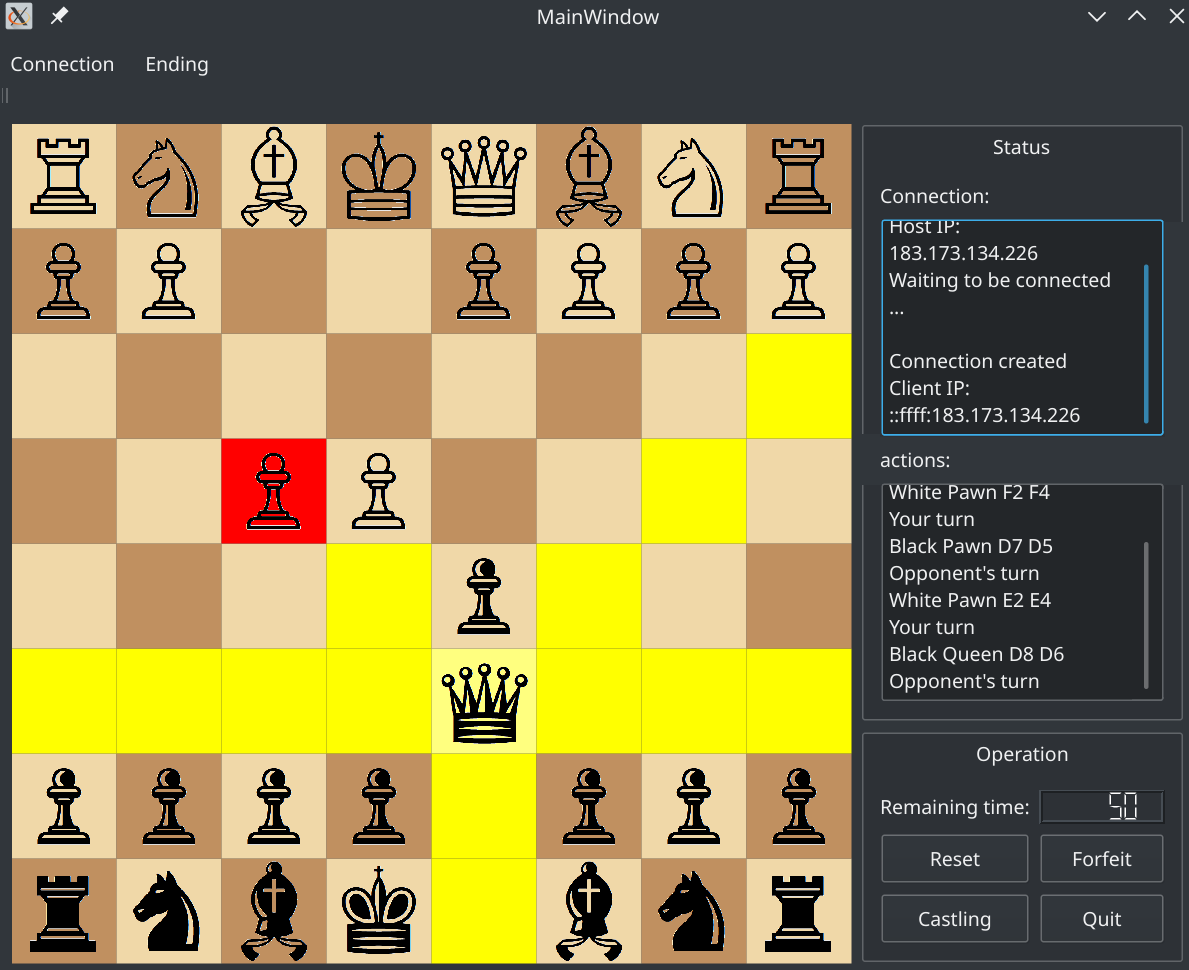
\includegraphics[width=.8\textwidth]{control.png}
                                \caption{操作}
                                \label{fig8}
                        \end{figure}


\section{程序架构}
        \subsection{通信协议}
                \subsubsection{协议}
                        使用通信协议为TCP
                \subsubsection{通信格式}
                        \begin{itemize}
                         \item 开局时若选择载入残局,服务端向客户端发送“Ending ”后跟残局文件内容,接着第二条信息发送服务端的颜色“Black”或“White”;若直接开始新局,则不会发送前缀“Ending”的信息,直接发送服务端的颜色
                         \item 过程中以棋谱方式进行信息传输,落子一方向对方传输“Color Type Position Target”格式的信息,先为移动的棋子颜色,再为种类,然后是此棋子所在位置和要移动到的位置。其中棋子种类为:
                                \begin{itemize}
                                 \item Pawn 兵
                                 \item Knight 骑士(马)
                                 \item Bishop 主教(象)
                                 \item Rook 战车(车)
                                 \item Queen 皇后
                                 \item King 王
                                \end{itemize}
                        位置使用棋谱记位法,
                         \item 特殊信息
                                \begin{itemize}
                                \item Forfeit 投降
                                \item Stalemate 逼和
                                \item Black/White Pawn postion target Type 兵升变为Type种类的棋子
                                \item Castling king's\_postion rook's\_postion 王车易位
                                \end{itemize}
                        \end{itemize}

        \subsection{程序结构}
                本程序主要使用QPainter类进行图形的绘制\par
                \begin{table}[htbp]
                \centering
                \begin{tabular*}{.9\textwidth}{cp{.6\textwidth}}
                \toprule[1.2pt]
                Class(or Struct)&\multicolumn{1}{c}{作用}\\
                \midrule
                Mainwindow&程序主界面、控制连接的服务端、客户端和两者之间的信息交互\\
                ChessBoard&继承自QWidget。画棋盘、棋盘逻辑、控制用户与棋盘的交互。有QList存储所有棋子\\
                ChessPiece&存储棋子种类、位置、颜色信息的结构体\\
                Parser&用于从文件读入残局和存储残局到文件\\
                \bottomrule[1.2pt]
                \end{tabular*}
                \end{table}
\end{document}
